% MODELO LATEX PARA TCC DO IFCE 
% ELABORADO POR CARINA TEIXEIRA DE OLIVEIRA
% SETEMBRO DE 2017

\documentclass[
12pt, % tamanho da fonte
openright, % capítulos começam em pág ímpar (insere página vazia caso preciso)
oneside, % para impressão somente frente. Oposto a twoside (frente e verso)
a4paper, % tamanho do papel. 
% 	% -- opções do pacote babel --
english,% idioma adicional para hifenização
%french,% idioma adicional para hifenização
%spanish,% idioma adicional para hifenização
brazil,	% o último idioma é o principal do documento
]{abntex2}

% ------------------------
% PACOTES
% Mapear caracteres especiais no PDF
\usepackage{cmap}
% Usa a fonte Latin Modern
\usepackage{times}			
% Selecao de codigos de fonte.
\usepackage[T1]{fontenc}		
% Codificacao do documento (conversão automática dos acentos)
\usepackage[utf8]{inputenc}		
% Indenta o primeiro parágrafo de cada seção.
\usepackage{indentfirst}		
% Controle das cores
\usepackage{color}				
% Inclusão de gráficos
\usepackage{graphicx}			
\usepackage{multicol}
\usepackage{multirow}
%capitulos
\usepackage{titlesec}
% Pacotes adicionais, usados apenas no âmbito do Modelo Canônico do abnteX2
% para geração de dummy text
\usepackage{lipsum}				
% Pacotes de citações
% Paginas com as citações na bibl
\usepackage[brazilian,hyperpageref]{backref}	 
% Citações padrão ABNT
\usepackage[alf]{abntex2cite}	
% CONFIGURAÇÕES DE PACOTES
% Configurações do pacote backref
% Usado sem a opção hyperpageref de backref
\renewcommand{\backrefpagesname}{Citado na(s) página(s):~}
% Texto padrão antes do número das páginas
\renewcommand{\backref}{}
%Define os textos da citação
\renewcommand*{\backrefalt}[4]{
	\ifcase #1 %
		Nenhuma citação no texto.%
	\or
		Citado na página #2.%
	\else
		Citado #1 vezes nas páginas #2.%
	\fi}

% ------------------------
% atalhos
\titulo{eJET – Uma Plataforma Web para Jogos
Educativos de Tabuleiro}
\autor{EDGAR DOS SANTOS OLIVEIRA}
\local{Brasil}
\data{11 de Dezembro de 2019}
\instituicao{Instituto Federal de Educação, Ciência e Tecnologia do Ceará}
\tipotrabalho{Trabalho de Conclusão de Curso (TCC)}
% O preambulo deve conter o tipo do trabalho, o objetivo, o nome da instituição e a área de concentração 
\preambulo{Modelo canônico de Relatório Técnico e/ou Científico em conformidade
com as normas ABNT apresentado à comunidade de usuários \LaTeX.}


% ------------------------
% Configurações de aparência do PDF final
% alterando o aspecto da cor azul
\definecolor{blue}{RGB}{41,5,195}
%informações do PDF
\makeatletter
\hypersetup{
    %pagebackref=true,
	pdftitle={\@title}, 
	pdfauthor={\@author},
    pdfsubject={\imprimirpreambulo},
	pdfcreator={LaTeX with abnTeX2},
	%pdfkeywords={abnt}{latex}{abntex}{abntex2}{relatório técnico}, 
	colorlinks=true,% false: boxed links; true: colored links
    linkcolor=blue,	% color of internal links
    citecolor=blue,	% color of links to bibliography
    filecolor=magenta, % color of file links
	urlcolor=blue,
	bookmarksdepth=4
}
\makeatother


% ------------------------
% Espaçamentos entre linhas e parágrafos 
% O tamanho do parágrafo é dado por:
\setlength{\parindent}{1.5cm}
% Controle do espaçamento entre um parágrafo e outro:
\setlength{\parskip}{0.2cm}  % tente também \onelineskip

% compila o indice
\makeindex
%\input{modeloCapitulos}

\begin{document}

%PARA UTILIZAR ARIAL
\fontfamily{phv}  %fonte Arial
\renewcommand{\rmdefault}{phv}      

% Retira espaço extra obsoleto entre as frases.
%\frenchspacing 
\thispagestyle{empty}
\vfill
\begin{center}

\begin{figure}[t]
\centering

\includegraphics[width=4cm]{figuras/ifce-ceara.png}%\\[-0.01in]
\end{figure}
\vspace{0.5 cm}
{\normalsize\bfseries INSTITUTO FEDERAL DE EDUCAÇÃO, CIÊNCIA E TECNOLOGIA DO CEARÁ} \\
{\normalsize\bfseries IFCE CAMPUS ARACATI} \\
{\normalsize\bfseries COORDENADORIA DE CIÊNCIA DA COMPUTAÇÃO}  \\ 
{\normalsize\bfseries BACHARELADO EM CIÊNCIA DA COMPUTAÇÃO}  \\ 

\vspace*{1in}
\begin{large} \bfseries \imprimirautor \end{large}\\[0.4in]

\vspace*{4cm}
\noindent \\
\large\bfseries{eJET – Uma Plataforma Web para Jogos
Educativos de Tabuleiro)} \\
\vfill
\normalsize\bfseries{ARACATI-CE\\ANO DE PUBLICAÇÃO}

\end{center}
\normalsize
\vfill
\begin{center}

{\imprimirautor\\}
\vspace{3cm}
{\textsc{eJET – Uma Plataforma Web para Jogos
Educativos de Tabuleiro}\\}
\vspace{5cm}
\hspace{.45\linewidth}
\begin{minipage}{.50\linewidth}
Trabalho de Conclusão de Curso (TCC) apresentado ao curso de Bacharelado em Ciência da Computação do Instituto Federal de Educação, Ciência e Tecnologia do Ceará - IFCE - Campus Aracati, como requisito parcial para obtenção do Título de Bacharel em Ciência da Computação.

\vspace{0.5 cm}

Orientador (a): Prof. <Ricardo L.> Ricardo Lenz

\end{minipage}

\vspace{2cm}
\vfill
{\large Aracati-CE\\ANO DE PUBLICAÇÃO}

\end{center}

%\begin{fichacatalografica}
	\sffamily
	\vspace*{\fill}					% Posição vertical
	\begin{center}					% Minipage Centralizado
	\fbox{\begin{minipage}[c][8cm]{13.5cm}		% Largura
	\small
	\imprimirautor
	%Sobrenome, Nome do autor
	
	\hspace{0.5cm} \imprimirtitulo  / \imprimirautor. --
	\imprimirlocal, \imprimirdata-
	
	\hspace{0.5cm} \pageref{LastPage} p. : il. (algumas color.) ; 30 cm.\\
	
	\hspace{0.5cm} \imprimirorientadorRotulo~\imprimirorientador\\
	
	\hspace{0.5cm}
	\parbox[t]{\textwidth}{\imprimirtipotrabalho~--~\imprimirinstituicao,
	\imprimirdata.}\\
	
	\hspace{0.5cm}
		1. Palavra-chave1
		2. Palavra-chave2.
		2. Palavra-chave3.
% 		I. Emanuel Bezerra Rodrigues.
% 		II. Instituto Federal de Educação, Ciência e Tecnologia do Ceará - Campus Aracati.
% 		III. Coordenadoria de Ciência da Computação.
% 		IV. Título da dissertação			
	\end{minipage}}
	\end{center}
\end{fichacatalografica}
\begin{folhadeaprovacao}
\vfill
\begin{center}

{NOME COMPLETO DO AUTOR\\}
\vspace{1.5cm}
{\textsc{TÍTULO DO TRABALHO: SUBTÍTULO (se houver)}\\}
\vspace{1.5cm}
\hspace{.45\linewidth}
\begin{minipage}{.50\linewidth}
Trabalho de Conclusão de Curso (TCC) apresentado ao curso de Bacharelado em Ciência da Computação do Instituto Federal de Educação, Ciência e Tecnologia do Ceará - IFCE - Campus Aracati, como requisito parcial para obtenção do Título de Bacharel em Ciência da Computação. 
\end{minipage}
\vspace{1.0 cm}

\end{center}

\noindent\\
{Aprovada em <data>}

\vspace{1.5 cm}
\begin{center}
{BANCA EXAMINADORA}
\assinatura{Prof. <Título Abreviado> <Nome completo> (Orientador (a)) \\ 
<instituição>}
\assinatura{Prof. <Título Abreviado> <Nome completo> (Orientador (a)) \\<instituição>}
\assinatura{Prof. <Título Abreviado> <Nome completo> (Orientador (a)) \\<instituição>}

\end{center}
\end{folhadeaprovacao}
\vfill
\begin{center}
{\textbf{DEDICATÓRIA}\\}
\end{center}

\noindent Aos meus pais.\\
\noindent Aos mestres.\\


\vfill
\begin{center}
{\textbf{AGRADECIMENTOS}}
\end{center}

Agradecimentos aqui.



\vfill
\begin{center}
{\textbf{RESUMO}\\}
\end{center}
\noindent

Os jogos são uma ferramenta muito comum na educação, porém o desenvolvimento dessa ferramenta ainda pode ser um processo difícil e confuso que cria dúvidas de qual a melhor tecnologia a ser utilizada. Este artigo apresenta o processo de desenvolvimento e funcionamento  de um \textit{framework} para a criação de jogos educativos na Web com Canvas e SVG. Aproveitando a oportunidade disponibilizada por esta ferramenta torna-se possível fazer um comparativo de ambas tecnologias em diversos casos. A principal contribuição deste artigo é facilitar a criação de jogos educativos, mais especificamente jogos de tabuleiro na língua portuguesa. O funcionamento dessa ferramenta servirá para orientar desenvolvedores de jogos a usar este instrumento em suas criações. Por último, o comparativo que será feito do desempenho do Canvas e SVG servirá tanto àqueles que desejam criar seus próprios \textit{frameworks} de desenvolvimento Web, como também desenvolvedores interessados em usar este \textit{framework}, que  permite o uso de ambas tecnologias, a escolher qual solução se encaixa melhor em seus jogos e pode ser útil para qualquer outro que possua dúvidas entre o uso destas ferramentas.

\vspace{\onelineskip}
 \noindent
 \textbf{Palavras-chaves}: Primeira. Segunda. Terceira.

\vfill
\begin{center}
{\textbf{ABSTRACT}\\}
\end{center}

\noindent

Games are a very common tool in education, but the development of this tool can still be a difficult and confusing process that raises doubts as to which technology is the most suitable for a certain context. This article shows the process of development and working of a \textit{framework} for creating educational Web games with Canvas and SVG. Taking advantage of the opportunity provided by this tool, it is possible to make a comparison of both technologies in several cases. The main contribution of this article is to facilitate the creation of educational games, more specifically board games in the Portuguese language. The Working of this tool will guide game developers to use this tool in their creations. Finally, the comparison of the performance of Canvas and SVG will serve both those who wish to create their own Web game frameworks, developers interested in using this framework, which allows the use of both technologies, to choose which solution fits best in your games and  also can be useful to anyone who has questions.
 
 \vspace{\onelineskip}
    
 \noindent
 \textbf{Keywords}: First. Second. Third.

\vfill
\begin{center}
{\textbf{LISTA DE ILUSTRAÇÕES}}
\end{center}

\renewcommand\listfigurename{}
\listoffigures* % * indica que não aparecerá no sumário

\vfill
\begin{center}
{\textbf{LISTA DE TABELAS}}
\end{center}
\renewcommand\listtablename{}
\listoftables*
\vfill
\begin{center}
{\textbf{LISTA DE ABREVIATURAS E SIGLAS}}
\end{center}
\vspace{0.5cm}

\begin{siglas}
\item[IFCE] Instituto Federal de Educação, Ciência e Tecnologia do Ceará
\item[TCC] Trabalho de Conclusão de Curso
\end{siglas}

 \vfill
\begin{center}
{\textbf{SUMÁRIO}}
\end{center}

\renewcommand\contentsname{}
\tableofcontents*
\textual

%CAPITULOS
\chapter{INTRODUÇÃO}
\label{Introducao}

\section{Motivação}

%#1
A educação é um componente essencial da sociedade em que vivemos, este é um fator determinante para o desenvolvimento humano. Portanto a qualidade da educação disponível em um país é um forte indicativo do seu futuro, melhorando-o ou piorando-o. De acordo como  Global Partnership for Education, em um \textit{rank} educacional, o Brasil está em 55º com 528 pontos de distância do primeiro colocado. O Brasil possui 12 milhões de analfabetos e mais 50\% dos adultos entre 25 e 64 anos não concluíram o Ensino médio.

Atualmente os métodos de ensino tradicionais têm dificuldades para engajar e estimular seus estudantes. O uso de jogos como ferramenta auxilia no ensino e muitas vezes proporcionam resultados melhores \cite{Girard&Ecalle&Magnan:13}. Essa aplicação pode se apresentar através da \textit{gamification}, o uso de mecânicas e dinâmicas de jogos para engajar pessoas. Assim, para resolver problemas e melhorar o aprendizado ,  onde alguns aspectos base dos videogames são adaptados para outros cenários, como os pontos que  são uma estrutura básica em jogos \cite{Zichermann&Cunningham:11} usado com propósito de motivar o jogador e também mostrar o seu progresso na tarefa que está sendo realizada.

Brincar ou jogar é uma atividade natural durante a vida de inúmeros animais, incluindo o ser humano, principalmente durante a infância. Essa atividade naturalmente atrai os seres humanos e é fruto de um processo evolutivo. Os animais que jogam ou simulam atividades antes de realizá-las de fato possuem um desempenho melhor. Por tanto aprender brincando é o método natural de adquirir e reforçar o conhecimento \cite{Bekoff&DiMotta:08}.

Alguns professores podem interpretar jogos como um inimigo às suas aulas, porém os mesmos podem se tornar poderosos aliados. A assistência de computadores na educação é conhecida como uma ferramenta efetiva para melhorar o aprendizado tanto em adultos quanto em crianças, pois pode ser muito eficiente em prover engajamento nos estudos \cite{Girard&Ecalle&Magnan:13}.

%#2
Os jogos usados como ferramentas geralmente são chamados \textit{serios games}. Estes são capazes de aumentar o engajamento dos alunos, dando aos mesmos a possibilidade de aprender conteúdo teórico de forma divertida e no seu próprio ritmo, melhorando a qualidade do aprendizado em uma área específica. Existem diversas soluções para a criação de jogos, porém estas raramente são especificamente focadas em jogos educativos e não costumam ser amigáveis, principalmente para não falantes da língua inglesa.

Como \cite{liu2013effect} em [\textit{ The Effect of Game-Based Learning on Students}] mostram um estudo feito com crianças do jardim de infância. Os alunos que tiveram uma aula com auxílio de \textit{gamification}, como jogos e aplicativos, mostraram resultados melhores. Portanto \textit{gamefication} pode ser um poderoso aliado, mas criar ferramentas educativas pode se mostra um desafio \cite{liu2013effect}.

A Web é uma plataforma muito comum para jogos educativos, pois apesar de ainda não possuírem a
mesma capacidade gráfica que os jogos nativos, possuem vantagem em distribuição. Qualquer um
pode ter acesso usando o dispositivo e sistema operacional que achar mais confortável, esse 
aspecto é muito mais importante que eficiência no que diz respeito à educação, além de permitir
atualizações sem nenhum esforço do usuário \cite{Mills:19}.

Desenvolver um jogo de tabuleiro para \textit{Web} pode se tornar muito complexo, principalmente para pessoas inexperientes. Para auxiliar no desenvolvimento de jogos educativos é preferível o uso de ferramentas como \textit{frameworks}, que são capazes de facilitar a criação do aplicativo. Estes \textit{frameworks} devem criar automaticamente as partes comuns do projeto, deixando assim que o criador faça apenas aquilo que é necessário, para que o jogo se ajuste as necessidades da matéria a ser ensinada. Por consequência a ferramenta permitirá ao usuário criar conteúdo original, interativo, dinâmico. Sem \textit{frameworks} todos esse aspectos se tornam, muitas vezes, difíceis de serem implementados. Portanto um \textit{framework} contendo partes que pudessem ser desenvolvidas com uma ferramenta de software, além da programação de código,seria muito mais desejável ainda.

%#TODO
%Adicionar então: 
%(4) Delimitação do tema → jogos de tabuleiro que possam ser usados para ensino e diversão, usando sistemas computacionais leves (isto é, não precisa de CPU e GPU de última geração!).
%(5) Fazer comentário sobre objetivo de ser fácil e ter além do framework/código uma ferramenta:

\section{Objetivos}

Nesta secção serão abordados o objetivos, almejado neste trabalho, de duas forma objetivo geral e específicos.

\subsection{Objetivo Geral}

O trabalho pretende fornecer um \textit{framework} para desenvolvimento de jogos educativos leves de tabuleiro com gráficos 2D usando tecnologia Web. O \textit{framework} envolverá tanto uma base de código como ferramentas de software adicionais para facilitar o seu uso.


\subsection{Objetivos Específicos}

%#TODO:
%(1) Introduzir os principais conceitos teóricos relacionados a um framework de jogos gráficos 2D;(OBS: ver seção 2.1. mais adiante pra essa parte – que você vai fazer)

%(2) Introduzir os principais conceitos tecnológicos relacionados a um framework de jogos gráficos 2D;(OBS: ver seção 2.2 mais adiante para essa parte – que você já fez)

%(3) Apresentar uma investigação sobre frameworks relacionados de jogos para Web;(OBS: isso você já fez: Phaser, PixiJS, Kiwi.js, CreateJS, Construct, iLearnTest, análise geral; isso tudo ficará na Seção 3)

%(4) Implementar o framework para jogos educativos de tabuleiro (código);(OBS: isso já tem sido feito ao longo do tempo; precisa agora colocar no TCC trechos do seu código)

%(5) Implementar as ferramentas de software do framework;(6) Implementar um exemplo prático onde se aplica o framework, demonstrando assim suascapacidades;(OBS: isso já tem sido feito ao longo do tempo; você pode colocar screenshots do exemplo (demo)com breves explicações das telas e um pouco do código que utilizou pra o demo]


Esse objetivo aqui almejado deve ser alcançado através de um ferramenta simples e intuitiva, que seja capaz de entregar jogos de tabuleiro, como o mini de esforço por parte do desenvolvedor. Aquele que optar pela uso deste mecanismo, deverá desfrutar de um processo de criação onde fora suas preocupações apenas no conteúdo educacional que desejar apresentar através do jogo, pois o desenvolvimento será feito baseando-se em templates, logo o criador não terá maiores preocupações com as mecânicas do jogo. Por fim, se necessário ou desejável o usuário deste equipamento poderá modificar parte central da tecnologia, portanto podendo descomplicadamente, com pouca alterações em seu código, fazer uso de Canvas ou SVG em sua aplicação.

\section{Organização do Trabalho}

O restante desse trabalho é organizado da seguinte forma: na Seção 2 os conceitos teóricos e tecnológicosserão apresentados; na Seção 3, uma investigação sobre frameworks da área é apresentada; na Seção 4, aproposta de framework do presente trabalho é descrita; na Seção 5, as ferramentas do framework sãodescritas; na Seção 6, um exemplo (demo) é apresentado para ilustrar as capacidades do frameworkapresentado, com resultados e discussões; a Seção 7 apresenta as conclusões e opções de trabalhosfuturos. 
\chapter{Conceitos Preliminares}
\label{FundamentacaoTeorica}
%%
%Exemplo de referência bibliográfica \cite{abntex2-wiki-como-customizar}.

%Exemplo de uso de figura no Latex (Figura~\ref{fig:mafalda}).
%\begin{figure}[th]
%\centering{
%\caption{Legenda da Figura no topo.}
%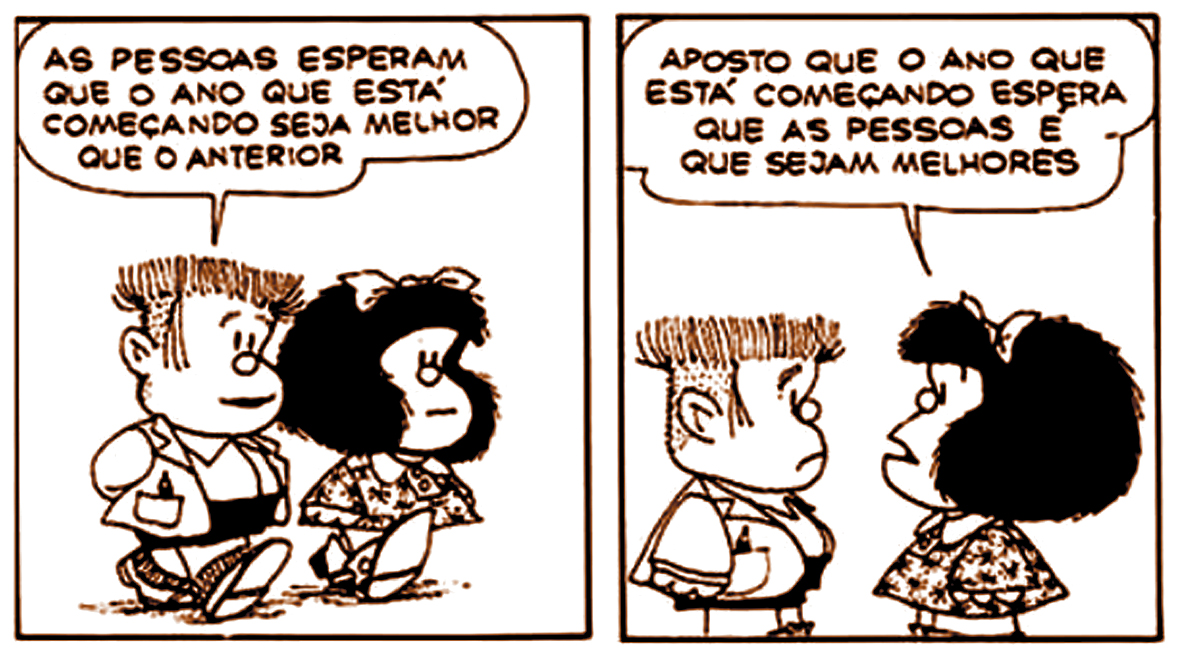
\includegraphics[width=0.75\textwidth]{figuras/mafalda}
%\begin{flushleft}
%\flushleft{Fonte: 
%Elaborado pelo autor.}
%\end{flushleft}
%\label{fig:mafalda}
%}
%\end{figure}


%Exemplo de uso de tabela no Latex (Tabela~\ref{tab:tabelaModelo}). Ver página 72 do Manual de Normalização de Trabalhos Acadêmicos do IFCE.
%\begin{table}[th]
%\centering
%\caption{Legenda da Tabela no Topo.}
%\label{tab:tabelaModelo}
%\begin{tabular}{llll}
%& Nota mínima & Nota máxima & Nota média\\\hline
%Ciências Humanas (CH)     & 324,8       & 862,1       & 546,5\\
%Ciências da Natureza (CN) & 330,6       & 876,4       & 482,2\\
%Linguagens e Códigos (LC) & 306,2       & 814,2       & 507,9\\
%Matemática (MT)           & 318,5       & 973,6       & 473,5\\ \hline  
%\end{tabular}
%\begin{flushleft}
%\flushleft{Fonte: 
%Instituto Brasileiro de Geografia e Estatística - IBGE.}
%\end{flushleft}
%\end{table}

Nessa subseção veremos uma  breve explicação de conceitos preliminares e tecnologias utilizadas. Isso será necessário para uma melhor compreensão dos Trabalhos Relacionados. 


\section{ Conceitos Teóricos }
Pode-se organizar o software de um jogo, num primeiro momento, em uma hierarquia de telas (screens). Assim, ao entrar num jogo, pode-se apresentar num determinado ponto uma tela inicial com um menu de opções (menu screen). O usuário poderá fazer algumas escolhas e configurações nesse momento inicial do jogo e depois escolher uma opção para iniciar o jogo, quando então se parte para a tela principal(main screen). Visualmente, pode-se realizar uma transição de uma tela para a outra (screen transition); existem diferentes animações gráficas para realizar esse tipo de transição, que normalmente envolve um movimento de saída da tela atual e o movimento de entrada da tela seguinte.

Uma vez na tela principal do jogo, geralmente há uma imagem de fundo (background image) que dá forma ao tabuleiro do jogo (board). O tabuleiro pode ser considerado como uma estrutura gráfica onde ocorre a “ação” propriamente dita do jogo. Há formas de construir a imagem do tabuleiro ou do fundo através de unidades gráficas menores chamadas de tiles. Os jogadores e demais personagens animados que possam haver no jogo são representados por objetos gráficos que se movem pelo cenário, sendo chamados de sprites. O movimento dos sprites que representam os jogadores tipicamente ocorre por um caminho pré-definido de posições no tabuleiro que será definido aqui como path.
Às vezes, o tabuleiro é grande demais para caber inteiramente de uma vez na tela. Nesse caso, pode-se focar somente uma certa área parcial do tabuleiro na tela. A área do tabuleiro que aparece na tela é controlada em função da posição da câmera. Assim, jogos gráficos com tabuleiros maiores poderão executar sem problemas mesmo em telas menores.

Geralmente, jogos de tabuleiro, por apresentarem uma dinâmica mais simples, apresentam os seus principais dados na tela, em painéis que indicam os pontos dos jogadores, isto é, o score da partida. Além disso, precisa ser indicado na tela de quem é o turno atual de jogada, já que nesses jogos a execução é tipicamente encadeada na forma de turnos (turn-based games). Pode-se chamar de estado atual do jogo (game state) o conjunto completo dessas informações: de qual jogador é o turno atual,todas as pontuações de cada jogador, a posição de cada um no tabuleiro e demais variáveis que controlam a situação atual do jogo.

Durante o jogo, a interface gráfica contará principalmente com movimentos dos sprites sobre o tabuleiro e eventuais caixas de diálogo (dialogs). Essas caixas de diálogo guiam o processo do jogo. No caso de jogos educativos de tabuleiro, podem trazer uma pergunta, as possibilidades de resposta do jogador, etc. Em muitos jogos, há o uso de algum tipo de fator aleatório para guiar o movimento do jogador,tipicamente realizado com a jogada de um dado (dice). Isso pode ser apresentado na forma de uma caixa de diálogo também.

Convém lembrar que a interface gráfica de muitos jogos é tipicamente controla via teclado. No caso de jogos para Web, é frequente a opção de controle por mouse também. Assim, deve-se ter o cuidado, em cada tela, de poder responder tanto pelo teclado quanto pelo mouse na medida em que isso for possível. No caso de uma tela de menu, pode-se ter um indicador visual (cursor) para definir em qual opção o usuário está atualmente selecionado. Caso o usuário simplesmente clique com o mouse numa outra opção, o cursor é colocado imediatamente ali e então a opção é ativada. Assim, mantém-se a devida harmonia no uso da aplicação.

Por fim, quando o jogo termina, uma tela final pode ser apresentada (ending screen). Nessa tela,tipicamente são apresentados os pontos finais de cada um e algumas estatísticas sobre a partida, como tempo ou número de acertos, erros, movimentos de um tipo ou outro, ou qualquer outra possibilidade de informação conforme admita o tipo do jogo.

Em toda a execução do jogo, do início ao fim, pode-se pressupor algum tipo de música de fundo(background music), com sons adicionais para cada ação (sounds), enriquecendo a experiência do jogador.

Uma observação que se sobressai diante da análise desses conceitos é que há uma estrutura relativamente comum a muitos jogos do gênero; essa estrutura não necessitaria, a princípio, de ter que ser completamente descrita por programação de código. Seria possível descrever parte dessa estrutura por meio de uma descrição mais simples, apropriada para uma automatização do desenvolvimento de jogos. Isso, de fato, é uma das contribuições do presente trabalho, que permitirá, conforme será visto mais adiante, descrever partes da estrutura do jogo como uma descrição textual num arquivo de simples personalização. Isso facilita a utilização do \textit{framework} proposto por outros educadores brasileiros que possam ter um conhecimento menos profundo na área de jogos, para que possam mais rapidamente montar um jogo que sirva ao propósito de diversão com aprendizado e enriquecimento cultural.

 \subsection{ Bitmap }

 O Bitmap é um formato padrão de imagem que contém uma matriz de \textit{pixels}, fornecendo a cor de cada pixel. Não contém informações geométricas sobre os objetos que estariam compondo a imagem, mas apenas a cor em cada pixel. Assim, esse formato não permite que a imagem possa ser esticada de forma a preservar as descrições geométricas dos objetos desenhados. É usado para fotos e outros tipos de desenho em que não é necessário esticar ou manipular partes.

\section{Conceitos Tecnológicos}

Considerando a proposta de desenvolvimento de jogos gráficos que utilizam tecnologias da Web, esta seção irá explicar algumas das principais tecnologias envolvidas nesse contexto. Algumas tecnologias no contexto de desenvolvimento na Web são opcionais: o desenvolvedor pode ou não utilizá-la. Os casos que foram avaliados como de uso mais frequente no desenvolvimento de jogos ou ainda que possam ter relevância perante o \textit{framework} sendo proposto neste trabalho foram selecionados para breves explicações aqui. Para maiores informações sobre cada uma das tecnologias sendo descritas à seguir, algumas referências são também apresentadas para o leitor consultar.

\subsection{ HTML }
 O HTML (Hypertext Markup Language) é a linguagem de marcação padrão de documentos que foram criados para serem exibidos em navegadores na Web. Ela é formada por blocos chamados \textit{tags}, esses blocos dão significado semântico ao conteúdo do documento, como por exemplo, a \textit{tag} 'p' dá o significado semântico de parágrafo ao conteúdo dentro dela, o conteúdo das \textit{tags} pode variar de texto, imagem e vídeo \cite{musciano1996html}.
 
 \subsection{ XML }
 
 %#4
 A Extensible Markup Language (XML), faz parte das SGMLs (Standard Generalized Markup Language), é um padrão para documentos de linguagens genéricas de marcação. Foi criada em 1998 pela XML Working Group, com o objetivo de ser usado diretamente na internet. Tecnicamente um documento XML é formado por entidades que podem se referir a outras entidades, sendo uma destas a entidade raiz, desta forma representando informações em um esquema similar a um grafo \cite{bray2000extensible}.
 
 \subsection{ CSS }

CSS  (Cascading Style Sheets) pode ser usada em conjunto com o HTML para descrever  como as informações contidas nas
\textit{tags} serão apresentadas. Ela foi criada para separar o conteúdo do estilo, cuidando de informações como
cores, posicionamento do conteúdo na página e quais
fontes usar para cada texto. Essa separação pode
ajudar na
acessibilidade e permitir flexibilidade às
páginas Web \cite{ahmadian2011desnutrin}.

 \subsection{ Javascript }

O Javascript é uma linguagem de programação de \textit{script} interpretada, como elementos de programação
orientada a objeto, criada com o objetivo de
tornar a página \textit{Web} dinâmica, definindo
seu comportamento e possibilitando a
interatividade com usuário
\cite{flanagan2006javascript}. Ela interage
diretamente com os outros pilares da
\textit{World Wide Web}: CSS e HTML.

\subsection{ Typescript }

O Typescript é uma linguagem que expande JavaScript. Foi criada com o objetivo de fazer o desenvolvimento de \textit{software} usando Javascript mais fácil em grandes escalas. Além disso essa extensão também possui alguns recursos que podem ser, com frequência, interessantes para um desenvolvedor, como tipagem de variáveis \cite{bierman2014understanding}.

 \subsection{ SVG }
 
 SVG  (Scalable Vector Graphics) é um formato de imagem vetorial para gráficos 2D baseado em XML  (Extensible Markup Language), uma linguagem de marcação
 \cite{ferraiolo2000scalable}. Ele possui suporte
 a interatividade e animações. Esse formato foi
 criado pela W3C (World Wide Web Consortium) desde
 1999 \cite{ferraiolo2000scalable}. O SVG pode se
 integrar às páginas Web através do HTML, com uso
 da \textit{tag} 'svg', oficialmente adicionada
 no HMTL5, os atributos pode ser estilizados
 através do CSS, como qualquer outro elemento de
 html5, e como uso do Javascript é possível criar animação e eventos interativos.
 
\subsection{ Canvas }
 
Canvas é um dos elementos do HTML que permite a renderização dinâmica de formas e  imagens \textit{bitmap}. Ele também
permite desenhar objetos 3D, com auxilio da WebGL (Web Graphics Library), uma biblioteca para renderização de gráficos 2D e 3D
no contexto das páginas Web \cite{shappir2012performing}.

\chapter{Frameworks de Jogos para Web}

\section{Delimitação da Pesquisa}

Conforme mencionado na Introdução, pretende-se trabalhar com jogos leves de tabuleiro. Nisso o presente trabalho pressupõe o gênero 2D de jogos gráficos, que é o mais frequente para esse tipo de jogo.Além disso, é desejável aqui que o jogo possa executar em uma variedade de sistemas computacionais,sem exigência de um equipamento mais caro. Isso significa que a natureza de jogo pretendida é tal que não se imponha o uso de uma CPU de última geração, ou grande quantidade de memória no sistema ou ainda uma GPU mais avançada. Portanto, o foco da pesquisa fica delimitado a uma execução mais leve no Browser. Observação: o termo “leve” pode ser considerado subjetivo – o que é leve para um usuário pode não ser leve para outro. Porém, a natureza gráfica 2D mais simples de jogos de tabuleiro já torna essa categorização mais simples, conforme se poderá inferir da própria apresentação dos frameworks à seguir.

\section{Framewroks}

\subsection{ Phaser }

Desenvolvido pela Photon Storm, Phaser é um
\textit{framework} gratuito e \textit{
open-source } para o desenvolvimento de jogos 2D
HTML5. Ele usa renderização com Canvas ou WebGL e
pode trocar entre eles automaticamente dependendo
do suporte do  \textit{browser}. Pode ser
compilado para IOS (iPhone Operating System),
Android e aplicações nativas com o uso de
\textit{Third-party software}, o desevolvedor
pode usar tanto Javascript como também Typescript
\cite{faas2017introduction}. 

O Phaser possuir um bom \textit{design}, é bem documentado, possui suporte e foi criado em com base no PixiJS, que será abordado posteriormente. Portanto, os principais problemas deste \textit{framework} são muitas vezes referentes à linguagem Javascript, para a qual o \textit{framework} for desenvolvido, fazendo com que frequentemente os desenvolvedores usem Typescript.

\subsection{ PixiJS }

O PixiJS (Pixi Javascript) é uma biblioteca, com estrutura de código muito similar ao ActionScript, de renderização que permite criar gráficos ricos e interativos, aplicações para múltiplas plataformas  e jogos sem a necessidade de um conhecimento profundo na WebGL ou lidar com compatibilidade de navegador e dispositivo. Caso o WebGL não seja suportado por alguma razão, o PixilJS é capaz de trocar para o uso do Canvas. Ela se torna uma biblioteca atrativa para usuários de ActionScript, por sua similaridade de estrutura. Segundo a Goodboy, empresa que o criou \cite{van2015learn}, o PixiJs tem como principal vantagem, a velocidade de renderização que faz com que muitas vezes ela seja utilizada por outros \textit{frameworks} com Phaser por exemplo \cite{van2015learn}.
Essa biblioteca realiza bem o que se propõe, renderização, mas apenas isso pode ser visto como muito pouco, na criação de jogos, em comparação a outros trabalhos também mostrados aqui.



\subsection{ Kiwi.js }


O Kiwi.js se trata de um  \textit{framework} 
\textit{open-sorce} para a criação de jogos HTML5
para \textit{desktop} e \textit{mobile}, com o
uso do  \textit{framework}  CocoonJS, que permite a construção de aplicativos \textit{mobile} a partir
de HTML5, CSS3 e Javascript, ao invés de usar
linguagens nativas como Java ou Swift, CocoonJS
usa um tipo de compressão de uma página Web
normal. 

Segundo seus desenvolvedores o Kiwi.js é
o  \textit{framework}  mais fácil e amigável
existente no momento, assim sendo o mais
recomendável para alguém que está começando. O maior problema encontrado no kiwi.js é o aparente abandono do projeto pelos desenvolvedores, o repositório do Github mostra que o último \textit{commit} realizado for feito em 2015 \cite{kiwiGit}.

\subsection{ CreateJS }

CreateJS (Create Javascript) é uma coleção de bibliotecas Javascript e ferramentas que funcionam juntas para criar conteúdo interativo na internet, podendo ser usada para a criação de jogos. Ela é composta por 4 módulos: EaselJS, TweenJS, SoundJS, PreloadJS \cite{manderscheid2014beginning}.

\paragraph{ EaselJS (Ease Javascript) }
O EaselJS fornece soluções para trabalhar com
gráficos e interatividade com o HTML5 Canvas. Ele fornece uma API que é familiar aos
desenvolvedores do Flash, incluindo uma lista de
exibição hierárquica \cite{manderscheid2014beginning}.

\paragraph{ TweenJS (Tween Javascript) }
TweenJS é uma biblioteca de interpolação para uso
em JavaScript. Foi desenvolvida para integrar-se
à biblioteca EaselJS, mas não depende dela. Ele
suporta interpolação de propriedades de objetos
numéricos e propriedades de estilo CSS \cite{manderscheid2014beginning}.

\paragraph{ SoundJS (Sound Javascript) }
O SoundJS (Sound Javascript) trata da reprodução de áudio via HTML5, WebAudio e Flash usando um modelo de plug-in, que consulta recursos e seleciona um plug-in adequado para funcionar em várias plataformas na maioria dos navegadores \cite{manderscheid2014beginning}.

\paragraph{ PreloadJS (Preload Javascript) }
PreloadJS (Preload Javascript) é uma biblioteca para pré-carrega ativos, incluindo imagens  (usando um modelo de plug-in e SoundJS), sons, JavaScript, dados de texto etc. Ele usa XHR (XMLHttpRequest) sempre que possível e volta ao carregamento baseado em \textit{tags}. Permite várias filas e várias conexões \cite{manderscheid2014beginning}.

\subsection{Construct}

Construct é um \textit{game engine} para criação de jogos 2d em HTML5, criado pela Scirra Ltd. Este possui propósito geral, não focado em uma modalidade de jogo. Permite a criação de jogos para não programadores, através da interface gráfica, porém os recursos oferecidos pela interface muitas vezes são inferiores ao que a programação direta pode oferecer. A empresa mantenedora do projeto passou a dar suporte a linguagem Javascript a partir do Construct 3 o que aumentou a acessibilidade proporcionada pela \textit{engine}, isto somado a uma comunidade ativa tornando-o uma das ferramentas mais usadas pelos desenvolvedores de jogos.

\subsection{iLearnTest}

%#3
O iLearnTest é um framework para a criação de jogos educativos, baseado em \textit{templates}. Durante o desenvolvimento do jogo, ele separa o conteúdo educativo das mecânicas do jogo incorporando o conteúdo, recebido através de um XML (Extensible Markup Language) e durante a jogatina permite ao estudante visualizar a pontuação conquistada  através de respostas corretas. O iLearnTest foi criado em cima do Construct2, uma plataforma de criação de jogos open-source, tendo como objetivo principal minimizar o tempo gasto e o conhecimento necessário para criar um jogo educativo.

\section{Análise Geral dos Frameworks}

Todos os trabalhos mostrados são \textit{frameworks} de propósito geral, logo não possuem foco em jogos educativos. Portanto perdem parte dos benefícios inerentes ao uso de um \textit{framework}, além de exigir mais conhecimento do desenvolvedor para suprir as lacunas deixadas pelos \textit{frameworks}. Por consequência se tornam menos amigáveis para desenvolvedores iniciantes e também acabam, frequentemente, não alavancando a produtividade dos criadores tanto quanto em comparação com os resultados obtidos pelo uso de um \textit{framework} específico.

\subsection{ Modalidades de Jogos Educativos }

Como Alan Amory, Kevin Naicker, Jacky Vincent and Claudia Adans mostram em "\textit{The use of computer games as an educational tool: identification of appropriate game types and game elements}" que estudandes do primeiro e segundo ano de biologia mostram mais afinidades com jogos de aventura e estratégia do que jogos de simulação \cite{jayakanthan2002application}. Estratégia é, muito frequentemente, um gênero usado por jogos educativos pela sua inerente versatilidade de conteúdo, que podem ser abordados e tem a  predisposição de fazer o jogador pensar \cite{milgrom1990rationalizability}.

Alguns modelos clássicos de jogos abrangidos pelo gênero estratégia são jogos de tabuleiro com peças, jogo da memória, jogo de cartas, caça palavras e quebra cabeça. Estes modelos clássicos são facilmente moldáveis para diversos contextos educacionais. Com o uso de um \textit{framework} focado em jogos educativos, criar uma ferramenta de ensino baseada nesses modelos tradicionais se torna muito mais fácil, amigável para pessoas inexperientes e com liberdade suficiente para adaptá-los às necessidades específicas.

O \textit{framework} aqui apresentado, mostrará sua capacidade através do modelo de jogo de tabuleiro com peças. A forma como será realizado estará disponível na próxima seção. 
\chapter{Proposta do Framework: eJET}

\section{Introdução}

O objetivo geral deste trabalho é fornecer um \textit{framework} para desenvolvimento de jogos educativos leves de tabuleiro com gráficos 2D usando tecnologia Web, conforme delineado na Seção 1. Assim, um \textit{framework} foi   implementado   visando   mapear   cada   conceito   teórico   (ver   Seção   2.1)   num   código,organizado de forma estrutural em módulos. O  \textit{framework} proposto como um todo foi chamado de Framework Edgar de Jogos Educativos de Tabuleiro (eJET). Na sequência são apresentados os diferentes módulos que compõem o eJET e alguns trechos de código dos mesmos.

\section{Módulos do eJET}

\subsection {Módulo Screen: tela do logotipo, tela do menu, tela do jogo, tela de fim-de-jogo e transições de tela}

\subsection{ Módulo Menu: descrição hierárquica de menu navegável por teclado e mouse}

\subsection{ Módulo Board: imagem de fundo, câmera, tabuleiro e caminho (path) dos jogadores}

\subsection{ Módulo Sprite: objetos gráficos representando jogadores e seres animados}

\subsection{ Módulo Dialog: janela do tipo mensagem, questão-e-resposta e lançamento-de-dados}

\subsection{ Módulo Players: registro dos nomes dos jogadores, o turno atual, suas posições e pontuações (scores)}

%A proposta é mostrar uma ferramenta que auxilia na criação de jogos, especificamente jogos educativos na plataforma \textit{Web}. A \textit{Web}, do ponto de vista de uma plataforma para jogo, já possui muitos \textit{frameworks} capazes de suprir as necessidades de desenvolvedores experientes de jogos convencionais, porém eles não se propõem a educação. Para desenvolvedores inexperientes, como professores não ligados a área de tecnologia, pode ser muito difícil criar um jogo educativo para auxiliar nas aulas ou qualquer outra razão que seja.

%Pensar em quantidade de quadro por segundo, renderização, como realizar animações ou até mesmo a mecânica do jogo não deverão ser a preocupação principal no desenvolvimento de um jogo educativo, ao invés disso o foco deve ser mantido no conteúdo educativo. Portanto o \textit{framework}, mostrado aqui, é baseado em Template fazendo com que o usuário crie sobre uma base sólida de modelos de jogo baseado no gênero de estratégias.

%Um Template dar ao usuário estrutura básica do modelo de jogo do qual o Template pertente abranger, um tipo peça por exemplo em um Template para jogos de tabuleiro com peças. O usuário pode alterar o comportamento dos componentes da tela através de eventos, movendo uma peça para uma posição do tabuleiro ou removendo-a. Logo o \textit{framework} se encarregará de cuidar de todo os detalhes que estão por trás da configuração descrita pelo usuário, animando a movimentação das peças.


%Em cada Template há estrutura genérica para conter o conteúdo educativo que pretende ser mostrado no jogo. No caso de um jogo de tabuleiros com peças é possível inserir perguntas e respostas que serão mostradas quando uma peça estiver em uma determinada posição. É possível inserir o conteúdo educacional fora do padrão genérico com uso do eventos, demandando um pouco mais de esforço do criador, mas opcionalmente possibilitando a customização adaptativa para uma necessidade de ensino.

\chapter{Proposta das Ferramentas: eJET Tools}

\section{Introdução}

Além do \textit{framework} de código em si, o eJET contém duas ferramentas produzidas para auxiliar o desenvolvedor. Isso está em consonância com o contexto definido na Seção 1 de tentar facilitar desenvolvimento de jogos com o \textit{framework} na medida do possível e observando também a estrutura regular descrita na Seção 2 sobre jogos educativos de tabuleiro. Com base nisso, o trabalho avançou em duas frentes, gerando duas ferramentas que são descritas à seguir.

\section{Compilador eJET}

O Compilador eJET é um programa de linha de comando que recebe um arquivo com descrições da estrutura fundamental do jogo (telas, imagem e música de fundo, etc.) e gera um projeto completo com HTML, CSS e JavaScript pré-pronto para o desenvolvedor utilizar o framework eJET. O compilador aceita receber a descrição geral do jogo num formato XML / JSON / YAML.

O formato do arquivo de entrada é da seguinte maneira:

(decidir qual formato usar xml, json ou yaml)

\section{Editor de Tabuleiro do eJET}

O editor de tabuleiro do eJET é um software adicional que acompanha o \textit{framework} e permite a edição fácil da estrutura de caminho (path) que os jogadors seguem no tabuleiro. O software permite selecionar uma imagem de fundo e demarcar as coordenadas (X, Y) de cada posição possível no caminho que os jogadores poderão seguir na partida



 
 \chapter{Aplicação do Framework e Discussão de Resultados}

Uma proposta simples de jogo de tabuleiro educativo foi implementada para ilustrar as principaiscapacidades do framework proposto.

\label{Resultados}

 
 \chapter{Conclusão e Trabalhos Futuros}

Pesquisadores que atuam na área de educação estão sempre buscando um caminho contínuo de melhorias para  o  processo educacional.  Várias propostas  são feitas buscando mediar  um ensino mais  rico e produtivo   tanto   para   alunos   quanto   professores.   A   ideia   de   jogos   educativos   tem   se   estabelecido firmemente no cenário atual. Assim, o presente trabalho buscou se inserir dentro desse contexto, visando agregar mais opções para esse campo de atuação.

O objetivo geral do trabalho foi fornecer um esquema de desenvolvimento de jogos educativos de tabuleiro com tecnologias Web chamado eJET. O uso da plataforma Web para o trabalho permite um grande alcance de usuários; além disso, buscou-se um tipo de implementação que permitisse uma execução de jogos leves, que não exigissem hardware mais especializado. O processo de pesquisa foi conduzido primeiramente apresentando-se os principais conceitos teóricos da área e em seguida os conceitos   tecnológicos   envolvidos   na   implementação.   A   pesquisa,   em   seguida,   apresentou   uma investigação dos principais \textit{frameworks} disponíveis para a tarefa. Essa preparação conceitual-comparativa serviu finalmente de base para o próprio projeto sendo proposto, que envolveu tanto um \textit{frameworks} para programação com código quanto ferramentas (software) adicionais. Isso foi feito assim para cumprir os objetivos delineados no início do trabalho em relação à facilidade, a abrangência, o aproveitamento de estruturas regulares para automatização e o incentivo para mais pessoas utilizarem o eJET. Este próprio trabalho serve como introdução ao eJET para entusiastas na Internet, contendo tanto os conceitos quanto as instruções práticas, e adotando ainda o modelo de Software Livre para difusão aberta da tecnologia, convidando a todos para usar, contribuir e expandir o eJET.

Para trabalhos futuros, espera-se expandir o sistema desenvolvido aqui para incorporar partidas \textit{on-line} entre   jogadores  via   Internet   e   a  adequação  mais   automatizada   para   dispositivos  móveis,   além   da investigação de gráficos com WebGL para crescimento em termos de opções visuais.

\label{Conclusao}
 

% ELEMENTOS PÓS-TEXTUAIS
\postextual
% Referências bibliográficas
\bibliography{abntex2-modelo-references} 
\begin{apendicesenv}
	\partapendices
	\chapter*{APÊNDICE A - TÍTULO}
	\lipsum[5]
	\chapter*{APÊNDICE B - TÍTULO}
	\lipsum[5]
\end{apendicesenv}
 
\begin{anexosenv}
%Imprime uma página indicando o início dos anexos
	\partanexos
	\chapter*{ANEXO A - TÍTULO}
	\lipsum[10]
	\chapter*{ANEXO B - TÍTULO}
	\lipsum[10]
\end{anexosenv}
 


% INDICE REMISSIVO
%\printindex

\end{document}

